\chapter{مثال‌های عددی}
\label{ch:fasl4}
در این قسمت سه مسئله از مراجع معتبر برای بررسی صحت کد محاسباتی حل خواهند شد.


%----------------------------------------------------------------------------------------ی
%----------------------------------------------------------------------------------------ی
%                                      قسمت اوّل: مسئله اوّل
%----------------------------------------------------------------------------------------ی
%----------------------------------------------------------------------------------------ی
\section{مسئله اوّل}
این مسئله از \cite{vandujthes,vandujanal} انتخاب شده است. در این مسئله ناپیوستگی اشباع به خاطر ناهمگنی فشار مویینگی بررسی خواهد شد. هندسه مسئله از دوناحیه مجاور مطابق شکل \ref{fig:4vandujprob-geo} تشکیل شده‌است. در زمان $t=0$ ناحیه - پر از آب و ناحیه + پر از نفت است. این یعنی شرط اوّلیه برابر است با:
\begin{equation}
\label{eq:4ini}
S_0(x,y)=\begin{cases}
1 &x<0 \\
0 &x>0
\end{cases}
\end{equation}

به دلیل پدیده فشار مویینگی آب از ناحیه + به ناحیه - نفوذ خواهد کرد. برای مدل کردن این پدیده شرایط مرزی را مطابق جدول \ref{tab:4vanduj1} اعمال می‌کنیم. این شرایط به این معنی هستند که آبی از مرز‌‌ها به محیط متخلل تزریق نمی‌شود و دو فاز صرفا به خاطر پدیده مویینگی جابجا می‌شوند.

هندسه این مسئله در راستای $y$ متقارن است لذا این مسئله را یک بار با یک مش یک بعدی با ۱۲۰۰ نود و یک بار با یک مش بدون سازمان دو بعدی، مشابه آنچه در شکل \ref{fig:4vandujprob-mesh} نشان داده شده‌است و با ۴۰۰۰ نود و المان‌های مثلثی حل ‌می‌نماییم. 

خواص در نظر گرفته شده برای نواحی + , - و پارامتر‌های بدون بعد حاکم بر مسئله در جدول \ref{tab:4vanduj2} آمده‌اند. همانطور که مشاهده می‌کنید، دو حالت را برای توابع فشار مویینگی و تراوایی نسبی در نظر می‌گیریم. در یک حالت از توابع \text‌لاتین{vang} استفاده می‌نماییم. منحنی فشار مویینگی در این حالت از نوع \text‌لاتین{cc} است. در حالت دیگر از توابع \text‌لاتین{brooks} استفاده می‌نماییم که منحنی فشار مویینگی آن از نوع \text‌لاتین{cd} است و پدیده فشار ورودی در آن وجود دارد و فشار مویینگی می‌تواند در محل ناهمگنی پرش داشته باشد.

پروفیل‌های اشباع در $t=1$ در شکل \ref{fig:4vandujres} آمده‌اند. در هر دو حالت هماهنگی خوبی بین پاسخ ما و پاسخ نیمه‌تحلیلی \cite{vandujthes,vandujanal} مشاهده می‌شود. همانطور که انتظار داریم مقدار خطا در مش بدون سازمان دوبعدی از حالت مش یک‌بعدی بیشتر است.

%-------------------table boundary----------------------------------------------------------------%------------------------------------------------------------------------------------------------x
\begin{table}
\center
\caption{شرایط مرزی حاکم بر مسئله اوّل}
\begin{tabular}{|c|l|l|}
\hline
نام مرز & شرط مرزی اشباع  &شرط مرزی پتانسیل آب \\
\hline
مرز حاشور خورده
&$\Gamma_{SN}$ &\lr{ $\Gamma_{\varphi N}$ with $u_N = 0$ }\\
$\Gamma_L$ &\lr{$\Gamma_{SD}$ with $S_D = 1$} &\lr{$\Gamma_{\varphi N}$ with $u_N = -1$ }\\
$\Gamma_R$ &$\Gamma_{SN}$ &\lr{$\Gamma_{\varphi D}$ with $\varphi_D = 0$}  \\
\hline
\end{tabular}
\label{tab:4vanduj1} \\[1cm]
%-------------------table properties----------------------------------------------------------------
%------------------------------------------------------------------------------------------------x
\caption{خواص سنگ و پارامتر‌های بی‌بعد برای مسئله اوّل}
\begin{tabular}{|c |c |}
\hline
نام & مقدار \\
%
\hline
%
پارامتر‌های بی‌بعد
 &$\mathcal M = \mathcal N = \mathcal P = 1, \mathcal G = 0, \nabla h = (0,1)$ \\ 
%
\textbf{K}
&$-: \left[\begin{smallmatrix} 1 &0 \\ 0 &1 \end{smallmatrix}\right], \quad
 +: \left[\begin{smallmatrix} 0.25 &0 \\ 0 &0.25 \end{smallmatrix} \right]$ \\
%
$P_d$  	&$-:1 \quad +:2$ \\
%
$\phi$    &$-:1 \quad +:1$ \\
%
$k_r, J$  &\lr{\small $-,+:$ \pbox{6cm}{ case(I): brooks with $\lambda = 2$ \\[-2mm] case(II): vang with $m = 2/3$ } } \\
\hline
\end{tabular}
\label{tab:4vanduj2}
\end{table}


%-------------------figure for geometry----------------------------------------------------------%------------------------------------------------------------------------------------------------x
\begin{figure}
\begin{subfigure}{0.5\textwidth}
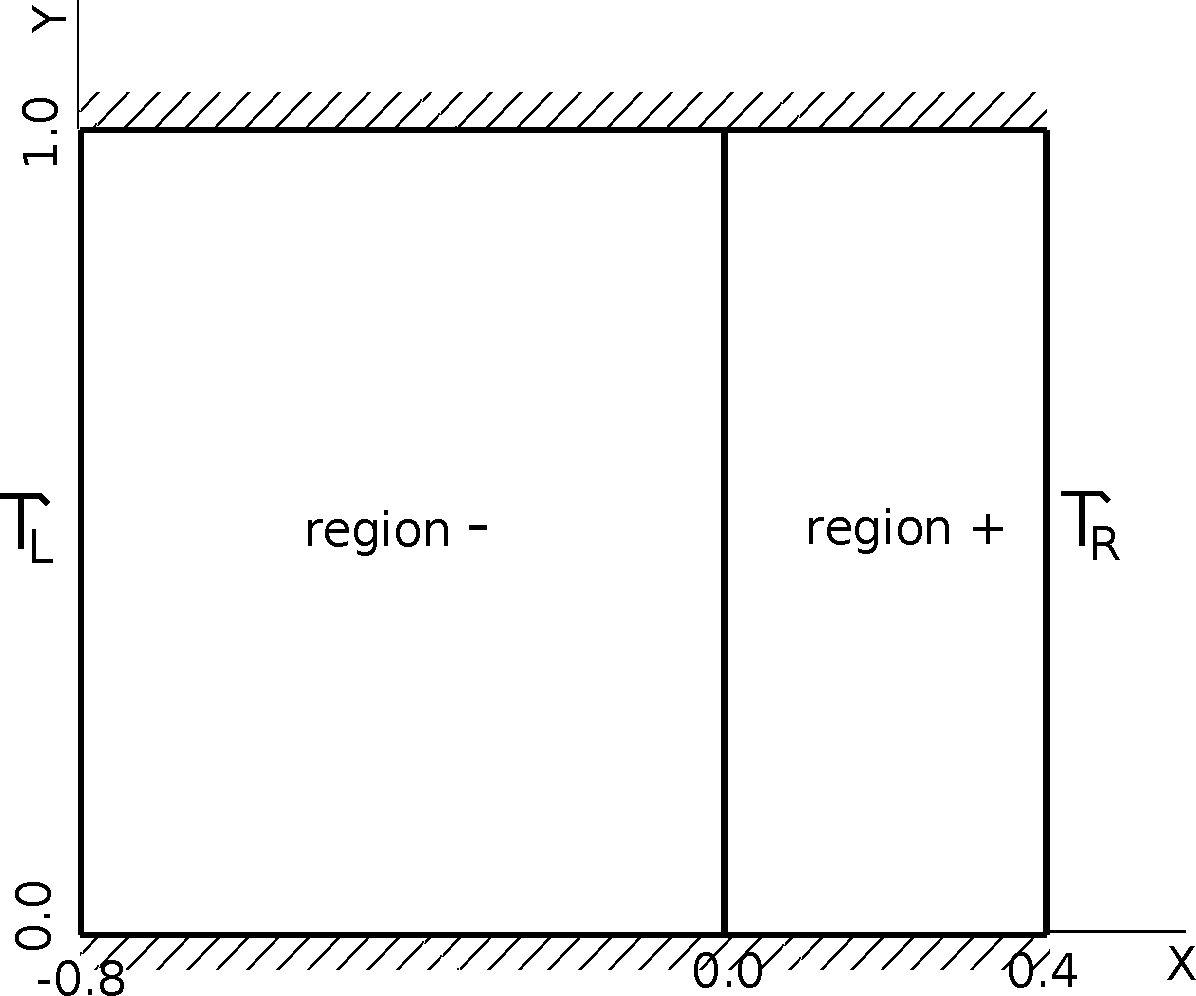
\includegraphics[width=.7\linewidth,center]{verif/vanduj-geom.pdf} 
\caption{هندسه مسئله}
\label{fig:4vandujprob-geo}
\end{subfigure}
\begin{subfigure}{0.5\textwidth}
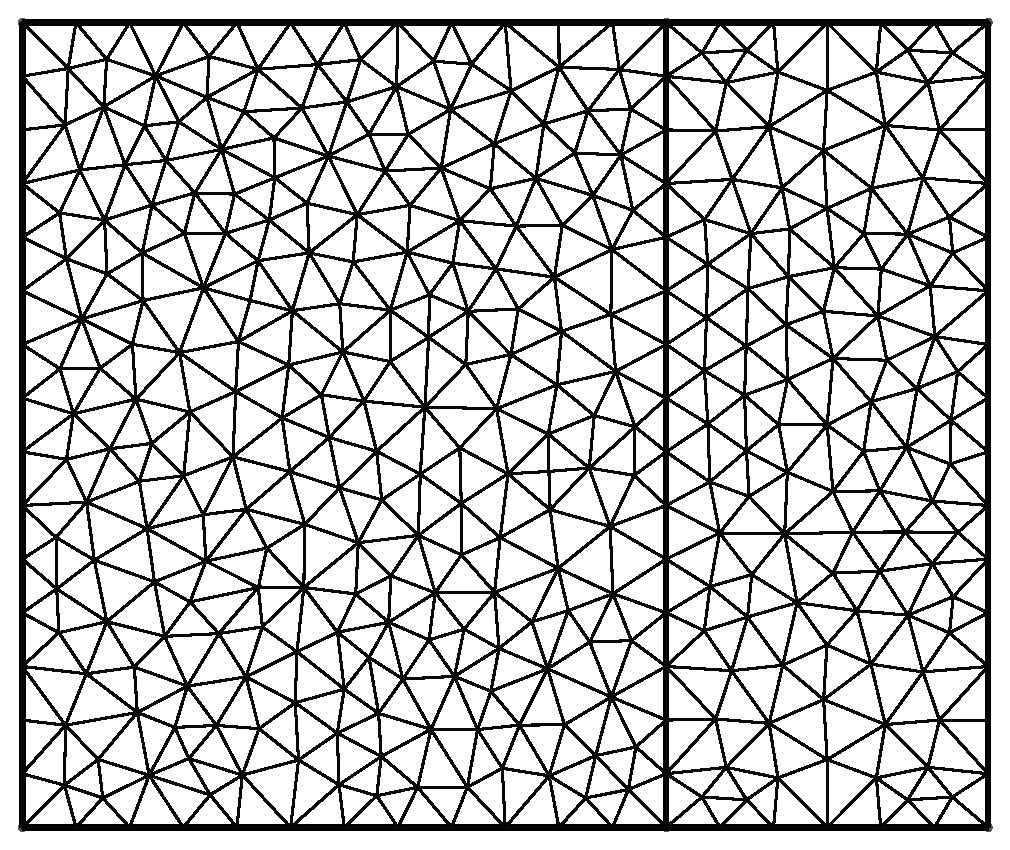
\includegraphics[width=.7\linewidth,center]{verif/vanduj-mesh.eps} 
\caption{نمونه مش دوبعدی}
\label{fig:4vandujprob-mesh}
\end{subfigure}
\caption[هندسه و مش مسئله اوّل]{هندسه و مش مسئله اوّل. همانطور که مشاهده می‌کنید هندسه در راستای محور $y$ متقارن است لذا می‌توان مسئله را در یک بعد نیز حل کرد. با توجه به اینکه مش ریز در چاپ مشخص نخواهد‌شد مشی که در قسمت (ب) نمایش داده‌ایم درشت‌تر از مشی است که برای حل مسئله استفاده کرده‌ایم.}
\label{fig:4vandujprob} \vspace{1cm}
%-------------------figure for answer----------------------------------------------------------
%--------------------------------------------------------------------------------------------x
\begin{subfigure}{0.5\textwidth}
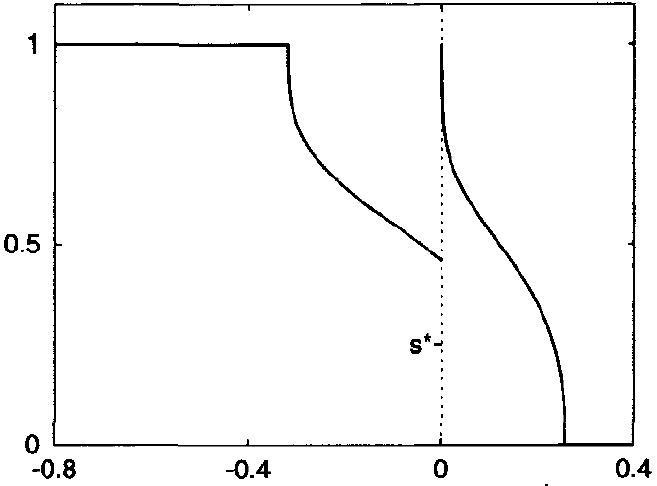
\includegraphics[width=.8\linewidth,center]{verif/vanduj-brooks.png} 
\end{subfigure}
\begin{subfigure}{0.5\textwidth}
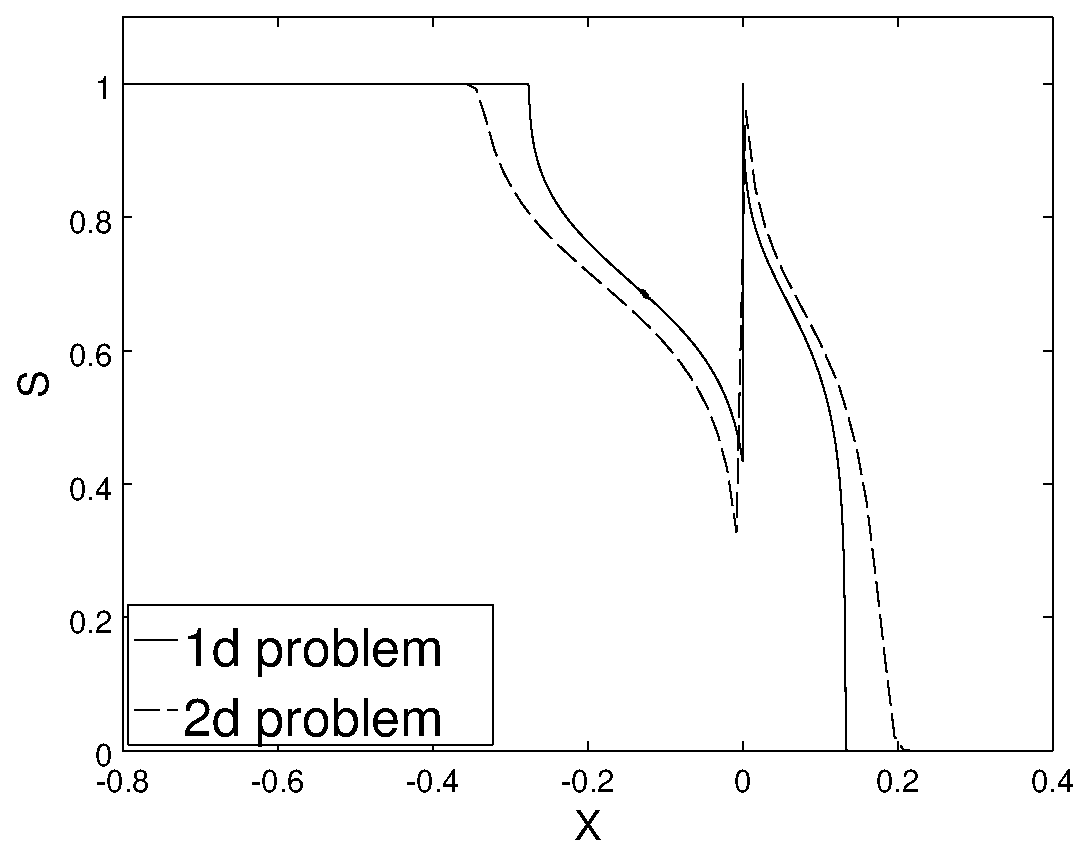
\includegraphics[width=.8\linewidth,center]{verif/vanduj-me-brooks.eps}
\end{subfigure}
\begin{subfigure}{0.5\textwidth}
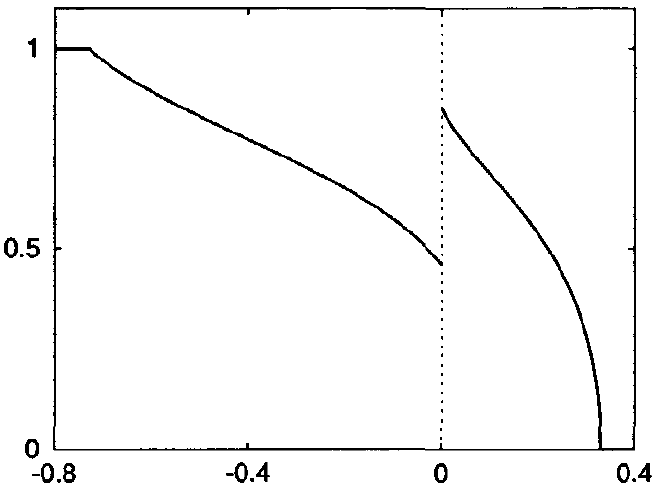
\includegraphics[width=.8\linewidth,center]{verif/vanduj-vang.png} 
\caption{پاسخ نیمه‌تحلیلی مراجع \cite{vandujanal,vandujthes}}
\label{fig:4vandujres-him}
\end{subfigure}
\begin{subfigure}{0.5\textwidth}
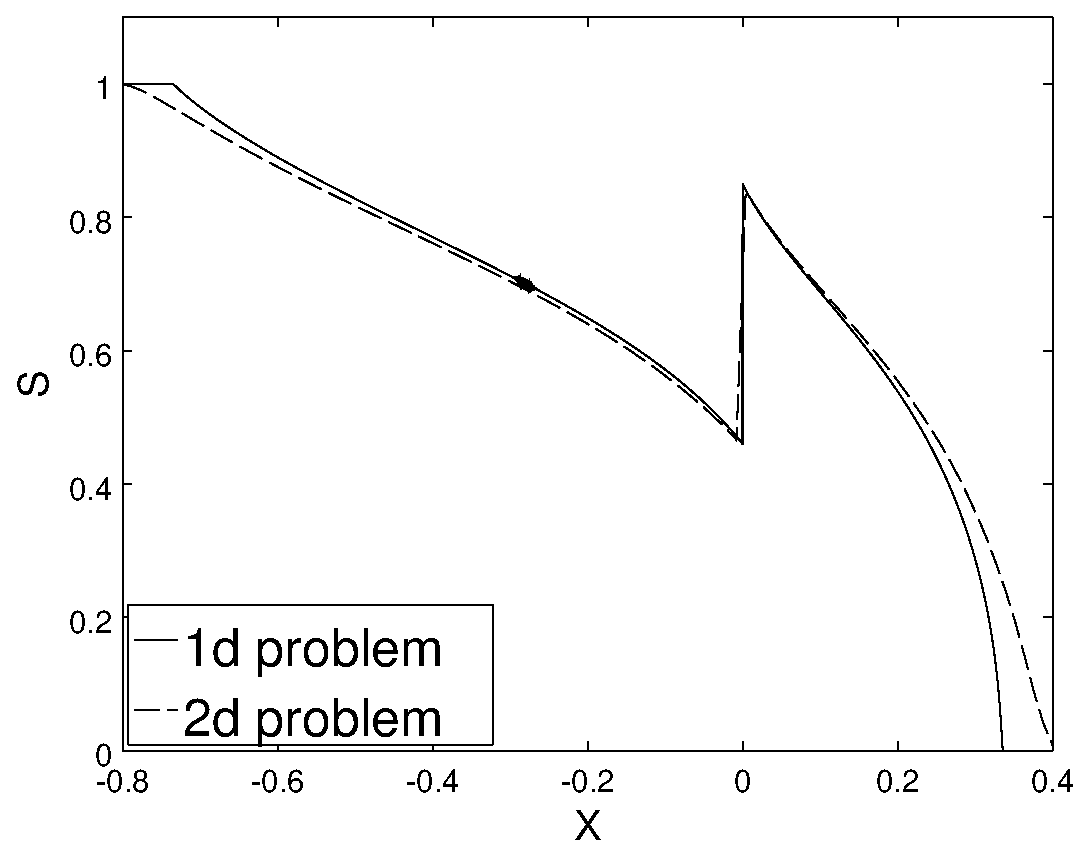
\includegraphics[width=.8\linewidth,center]{verif/vanduj-me-vang.eps} 
\caption{پاسخ محاسبه شده توسط روش این پروژه}
\label{fig:4vandujres-me}
\end{subfigure}
\caption[پروفیل اشباع روی خط $y=0.5$ در $t=1$ برای مسئله اوّل]{پروفیل اشباع روی خط $y=0.5$ در $t=1$ برای مسئله اوّل . در شکل‌های بالا از توابع تراوایی نسبی و فشار مویینگی \text‌لاتین{brooks} و در شکل‌های پایین از توابع \text‌لاتین{vang} استفاده شده است.  }
\label{fig:4vandujres}
\end{figure}
%----------------------------------------------------------------------------------------ی
%----------------------------------------------------------------------------------------ی
%                                      قسمت دوم: مسئله دوم
%----------------------------------------------------------------------------------------ی
%----------------------------------------------------------------------------------------ی
\section{مسئله دوم}
این مسئله از \cite{basthabil,bastn} انتخاب شده است و مدل کردن جاذبه را بررسی خواهد کرد. در این مسئله یک محیط متخلخل مطابق شکل \ref{fig:4peterprob} متشکل از دو ناحیه متفاوت وجود دارد. ناحیه ۱ تراوایی بالا و فشار مویینگی کم و ناحیه ۲ تراوایی کم و فشار مویینگی بالایی دارد. در $t=0$ تمام محیط از آب پر شده است: $S_0(x,y) = 1$. یک سیال \text‌لاتین{DNAPL}\footnote{Dense non-aqueous phase liquid. example: trichloroethylene or extra heavy crude oil} و سنگین‌تر از آب از مرز $\Gamma_T$ به محیط تزریق می‌شود و آب از دیگر مرز‌ها خارج می‌شوند. فشار در مرز $\Gamma_S$ از رابطه فشار هیدرواستاتیکی پیروی می‌کند، یعنی هندسه مسئله در این این مرز در مجاورت آب ساکن قرار دارد. به مرور زمان  \text‌لاتین{DNAPL} ناحیه ۱ را پر می‌کند ولی به دلیل فشار مویینگی بالای ناحیه ۲ نمی‌تواند وارد آن شود. دو حالت را برای فشار مویینگی ناحیه ۲ در نظر می‌گیریم. در یکی از این حالات \text‌لاتین{DNAPL} به هیچ وجه وارد ناحیه ۲ نمی‌شود ولی در حالت دیگر اندکی \text‌لاتین{DNAPL} وارد این ناحیه خواهد شد.

 در جدول \ref{tab:4peter1} شرایط مرزی مسئله مشخص شده است. پارامتر‌های بدون بعد و خواص سنگ‌ها به گونه‌ای انتخاب شده‌اند که بسیار به مقادیر داده شده در \cite{basthabil,bastn} نزدیک باشند. در جدول \ref{tab:4peter2} این مقادیر داده‌ شده‌اند. برای حل این مسئله از یک مش سازمان یافته $90\times 65$ استفاده شده‌است. 
 
 در شکل \ref{fig:4peterres} پروفیل اشباع برای هر دو حالت فشار مویینگی در $t=3500$ نمایش داده شده‌اند. همانطور که انتظار داشتیم زمانی که فشار مویینگی ناحیه ۲ کمتر است اندکی فاز \text‌لاتین{DNAPL} وارد آن می‌شود. نتایج به دست‌آمده هم‌خوانی خوبی با نتایج  \cite{basthabil,bastn}  دارند. هر چند در حالتی که ورود سیال به ناحیه ۲ را داریم اندکی تفاوت بین پاسخ‌ها مشاهده می‌شود.
 
 %-------------------table boundary----------------------------------------------------------------%------------------------------------------------------------------------------------------------x
\begin{table}
\center
\caption{شرایط مرزی حاکم بر مسئله دوم}
\begin{tabular}{|c|l|l|}
\hline
نام مرز & شرط مرزی اشباع  &شرط مرزی پتانسیل آب \\
\hline
مرز حاشور خورده
&$\Gamma_{SN}$ &\lr{ $\Gamma_{\varphi N}$ with $u_N = 0$ }\\
$\Gamma_T$ &\lr{$\Gamma_{SD}$ with $S_D=0$} &\lr{$\Gamma_{\varphi N}$ with $u_N=-5.14$} \\
$\Gamma_S$ &\lr{$\Gamma_{SD}$ with $S_D=1$} &\lr{$\Gamma_{\varphi D}$ with $\varphi_D=0$}  \\
$\Gamma_B$ &\lr{$\Gamma_{SD}$ with $S_D=1$} &\lr{$\Gamma_{\varphi N}$ with $u_N=0$}  \\
\hline
\end{tabular}
\label{tab:4peter1} \\[1cm]
%-------------------table properties----------------------------------------------------------------%------------------------------------------------------------------------------------------------x
\caption{خواص سنگ و پارامتر‌های بی‌بعد برای مسئله دوم}
\begin{tabular}{|c |c |}
\hline
نام & مقدار \\
%
\hline
%
پارامتر‌های بی‌بعد
 &$\mathcal M = 0.9, \mathcal N = 100, \mathcal P = 100, \mathcal G = 45.1, \nabla h = (0,1)$ \\ 
%
\textbf{K}
&$1: \left[\begin{smallmatrix} 66.4 &0 \\ 0 &66.4 \end{smallmatrix}\right], \quad
 2: \left[\begin{smallmatrix} 33.2 &0 \\ 0 &33.2 \end{smallmatrix} \right]$ \\
%
$P_d$  	&\lr{ $1: 755 \quad 2: $ case(I)$1466.1$ case(II)$1163.5$ }\\
%
$\phi$    &$1:0.360 \quad 2:0.343$ \\
%
$k_r$ &\lr{\small \pbox{6cm}{ $1:$ brooks with $\lambda = 2.7$ \\[-2mm] $2:$ brooks with $\lambda = 2$} } \\
$J$  &\lr{\small brooks with $\lambda = 2.5$ } \\
\hline
\end{tabular}
\label{tab:4peter2}
\end{table}

%-------------------figure for geometry----------------------------------------------------------%------------------------------------------------------------------------------------------------x
\begin{figure}
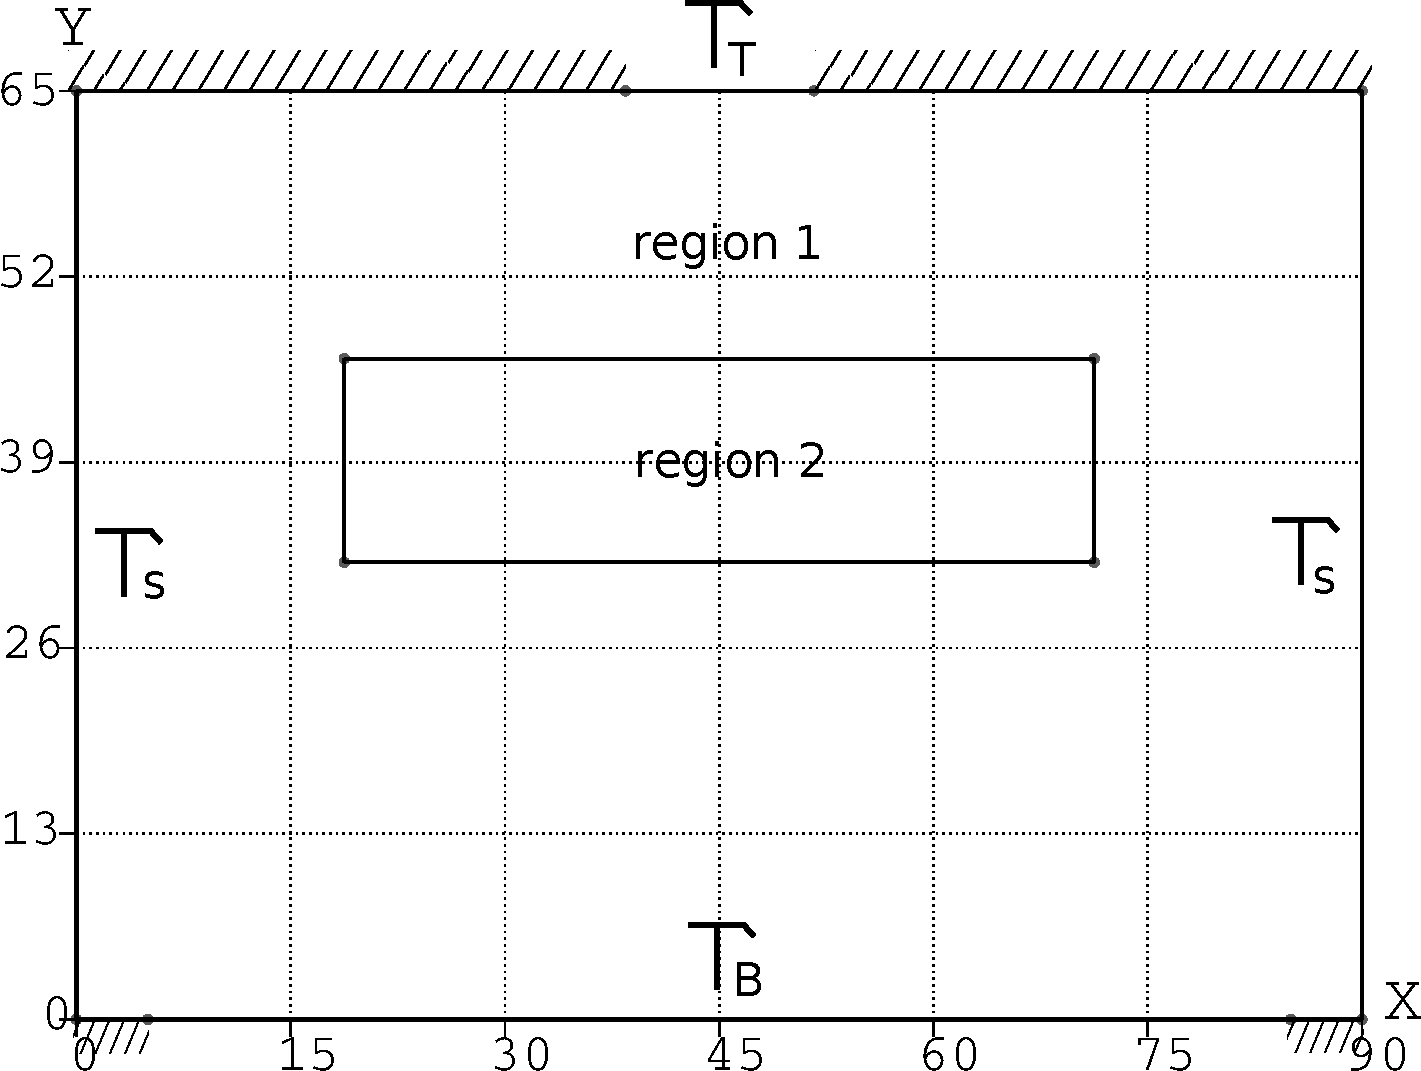
\includegraphics[width=.7\textwidth,center]{verif/peter-geom.pdf} 
\caption[هندسه مسئله دوم]{هندسه مسئله دوم. در این مسئله یک ناحیه با تراوایی کم در میان ماتریس اصلی قرار گرفته است. }
\label{fig:4peterprob} \vspace{1cm}
%-------------------figure for results----------------------------------------------------------%------------------------------------------------------------------------------------------------x
\begin{subfigure}{0.5\textwidth}
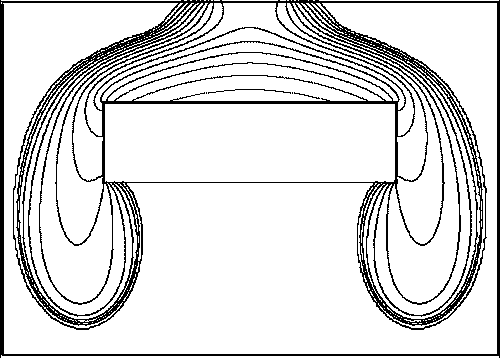
\includegraphics[width=.8\linewidth,center]{verif/peter-nopene.png} 
\end{subfigure}
\begin{subfigure}{0.5\textwidth}
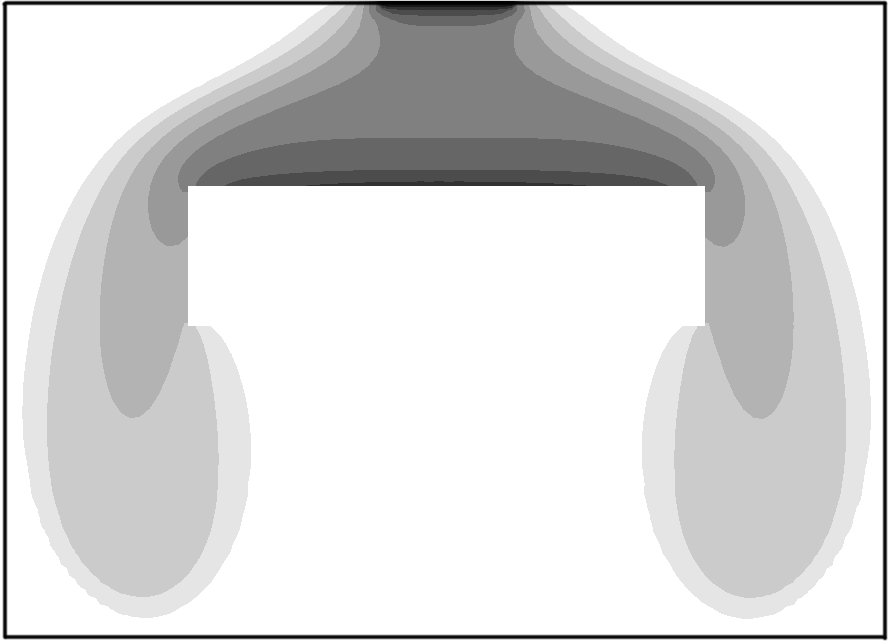
\includegraphics[width=.8\linewidth,center]{verif/peter-me-nopene.png}
\end{subfigure}
\begin{subfigure}{0.5\textwidth}
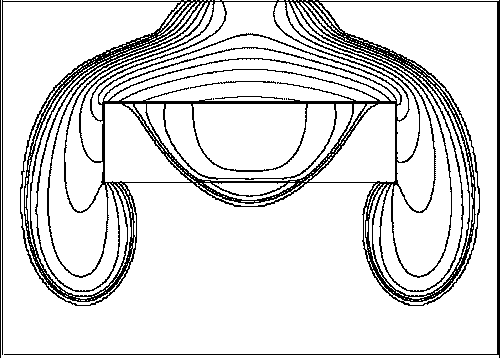
\includegraphics[width=.8\linewidth,center]{verif/peter-pene.png} 
\caption{پاسخ مراجع \cite{basthabil,bastn}}
\label{fig:4peterres-him}
\end{subfigure}
\begin{subfigure}{0.5\textwidth}
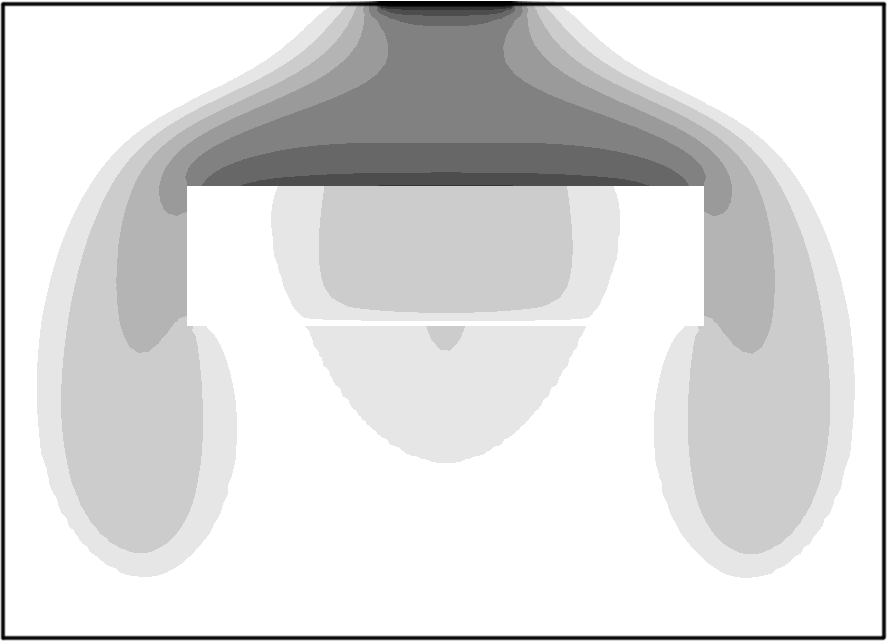
\includegraphics[width=.8\linewidth,center]{verif/peter-me-pene.png} 
\caption{پاسخ محاسبه شده توسط روش این پروژه}
\label{fig:4peterres-me}
\end{subfigure}
\caption[خطوط اشباع ثابت در $t=3500$ برای مسئله دوم]{خطوط اشباع ثابت در $t=3500$ برای مسئله دوم. در شکل‌های بالا مقدار $Pd$ برای ناحیه ۲ بیشتر از شکل‌های پایین است. در قسمت (ب) رنگ سیاه نشان دهنده بیشترین مقدار اشباع \text‌لاتین{DNAPL} و رنگ سفید نشان دهنده کمترین مقدار اشباع \text‌لاتین{DNAPL} هستند.}
\label{fig:4peterres}
\end{figure}

%----------------------------------------------------------------------------------------ی
%----------------------------------------------------------------------------------------ی
%                                      قسمت سوم: مسئله سوم
%----------------------------------------------------------------------------------------ی
%----------------------------------------------------------------------------------------ی
\section{مسئله سوم}
این مسئله از \cite{hoteitf,karimi1} انتخاب شده است. همانطور که در فصل \ref{ch:fasl1} اشاره کردیم، در \cite{karimi1} از روش گالرکین برای حل مسئله استفاده شده‌است. امّا در \cite{hoteitf} از روش المان محدود ترکیبی برای حل معادله فشار و از روش گالرکین گسسته برای حل معادله اشباع استفاده شده است و به دلیل \text‌لاتین{consrevative} بودن روش دوم و استفاده از \text‌لاتین{slope limiter}ها در آن، ادعا شده‌است که دقّت آن بالاتر و از مرتبه ۲ خواهد بود. پاسخ‌های دو مرجع اندکی متفاوت هستند لذا پاسخ‌های \cite{hoteitf} را برای مقایسه با پاسخ‌های خود انتخاب می‌کنیم.

 در این مسئله مدل‌سازی ترک‌ها را بررسی خواهیم کرد. هندسه مسئله در شکل \ref{fig:4firoozprob-geo} نمایش داده ‌شده‌است. در این مسئله ۶ ترک با تراوایی بسیار بالا و فشار مویینگی کم در محیط ماتریس قرار دارند که مختصات آن‌ها در همین شکل قابل مشاهده هستند. در $t=0$ تمام محیط متخلخل پر از نفت است $S_0(x,y) = 0$. آب از گوشه سمت چپ پایین به محیط تزریق شده و برداشت از گوشه سمت راست بالا انجام می‌شود. دو حالت را برای این مسئله در نظر می‌گیریم. در یک حالت فشار مویینگی در ترک و ماتریس صفر است ولی در حالت دیگر فشار مویینگی در هر دو محیط وجود دارد.

در جدول \ref{tab:4firooz2} شرایط مرزی مسئله مشخص شده‌اند. پارامتر‌های بدون بعد و خواص ماتریس و ترک به گونه‌ای انتخاب شده‌اند که بسیار به مقادیر داده شده در \cite{hoteitf} نزدیک باشند. در جدول \ref{tab:4firooz1} این مقادیر داده‌ شده‌اند. در این مسئله المان‌های چهارضلعی را نیز امتحان می‌کنیم. مش استفاده شده در شکل \ref{fig:4firoozprob-mesh} نمایش داده شده‌است.

در شکل \ref{fig:4firoozres} پروفیل اشباع برای هر دو حالت بدون و با فشار مویینگی بعد از تزریق آب به میزان ۲۵٪ و ۵۰٪ حجم خالی مخزن نمایش داده شده‌اند. زمانی که فشار مویینگی وجود داشته باشد آب دیرتر وارد ترک‌ها می‌شود و این امر باعث می‌شود که جبهه آب دیرتر به ناحیه برداشت برسد. در شکل \ref{fig:4firoozcurve} منحنی‌های تزریق-برداشت نمایش داده شده‌اند. رسیدن دیرتر جبهه آب به ترک‌ها که منجر به برداشت نفت بیشتر می‌شود در این منحنی‌ها نیز قابل مشاهده است. هماهنگی خوبی بین پاسخ به دست‌آمده در این پروژه و پاسخ‌های داده‌شده در \cite{hoteitf} وجود دارد. هر چند در حالتی که فشار مویینگی وجود نداشته باشد روش ما برداشت نفت را اندکی بیشتر پیش‌بینی می‌کند.

 %-------------------table boundary----------------------------------------------------------------%------------------------------------------------------------------------------------------------x
\begin{table}
\center
\caption{شرایط مرزی حاکم بر مسئله سوم}
\begin{tabular}{|c|l|l|}
\hline
نام مرز & شرط مرزی اشباع  &شرط مرزی پتانسیل آب \\
\hline
مرز حاشور خورده
&$\Gamma_{SN}$ &\lr{ $\Gamma_{\varphi N}$ with $u_N = 0$ }\\
نقطه تزریق
&\lr{$\Gamma_{SD}$ with $S_D=1$} &\lr{$\Gamma_{\varphi N}$ with $lu_N=0.02$ see eq. (\ref{eq:3bnd1}) } \\
نقطه برداشت
&$\Gamma_{SN}$ &\lr{$\Gamma_{\varphi D}$ with $\varphi_D=0$} \\
\hline
\end{tabular}
\label{tab:4firooz1} \\[1cm]
%-------------------table properties----------------------------------------------------------------%------------------------------------------------------------------------------------------------x
\caption{خواص سنگ و پارامتر‌های بی‌بعد برای مسئله سوم}
\begin{tabular}{|c |c |}
\hline
نام & مقدار \\
%
\hline
%
پارامتر‌های بی‌بعد
 &$\mathcal M = 0.45, \mathcal N = 198.2, \mathcal P = 198.2, \mathcal G = -1.35, \nabla h = (0,1)$ \\ 
%
\textbf{K}
&$m: \left[\begin{smallmatrix} 1 &0 \\ 0 &1 \end{smallmatrix}\right], \quad
 f:800000 $ \\
%
e
& $f:4\times10^{-6} $ \\
%
$P_d$  	&\lr{ m: case(I)$0$ case(II)$0.3$  f:  case(I)$0$ case(II)$0.04$ }\\
%
$\phi$    &$m:0.85 \quad f:0.17$ \\
%
$k_rw$ &\lr{\small $m: 0.2S^5 \quad f: S$ } \\
$k_rn$ &\lr{\small $m: 0.6(1-S)^3 \quad  f: 1-S$ } \\
$J$  &\lr{\small -ln(S) } \\
\hline
\end{tabular}
\label{tab:4firooz2}
\end{table}

%-------------------figure for geometry----------------------------------------------------------%------------------------------------------------------------------------------------------------x
\begin{figure}
\begin{subfigure}{0.5\textwidth}
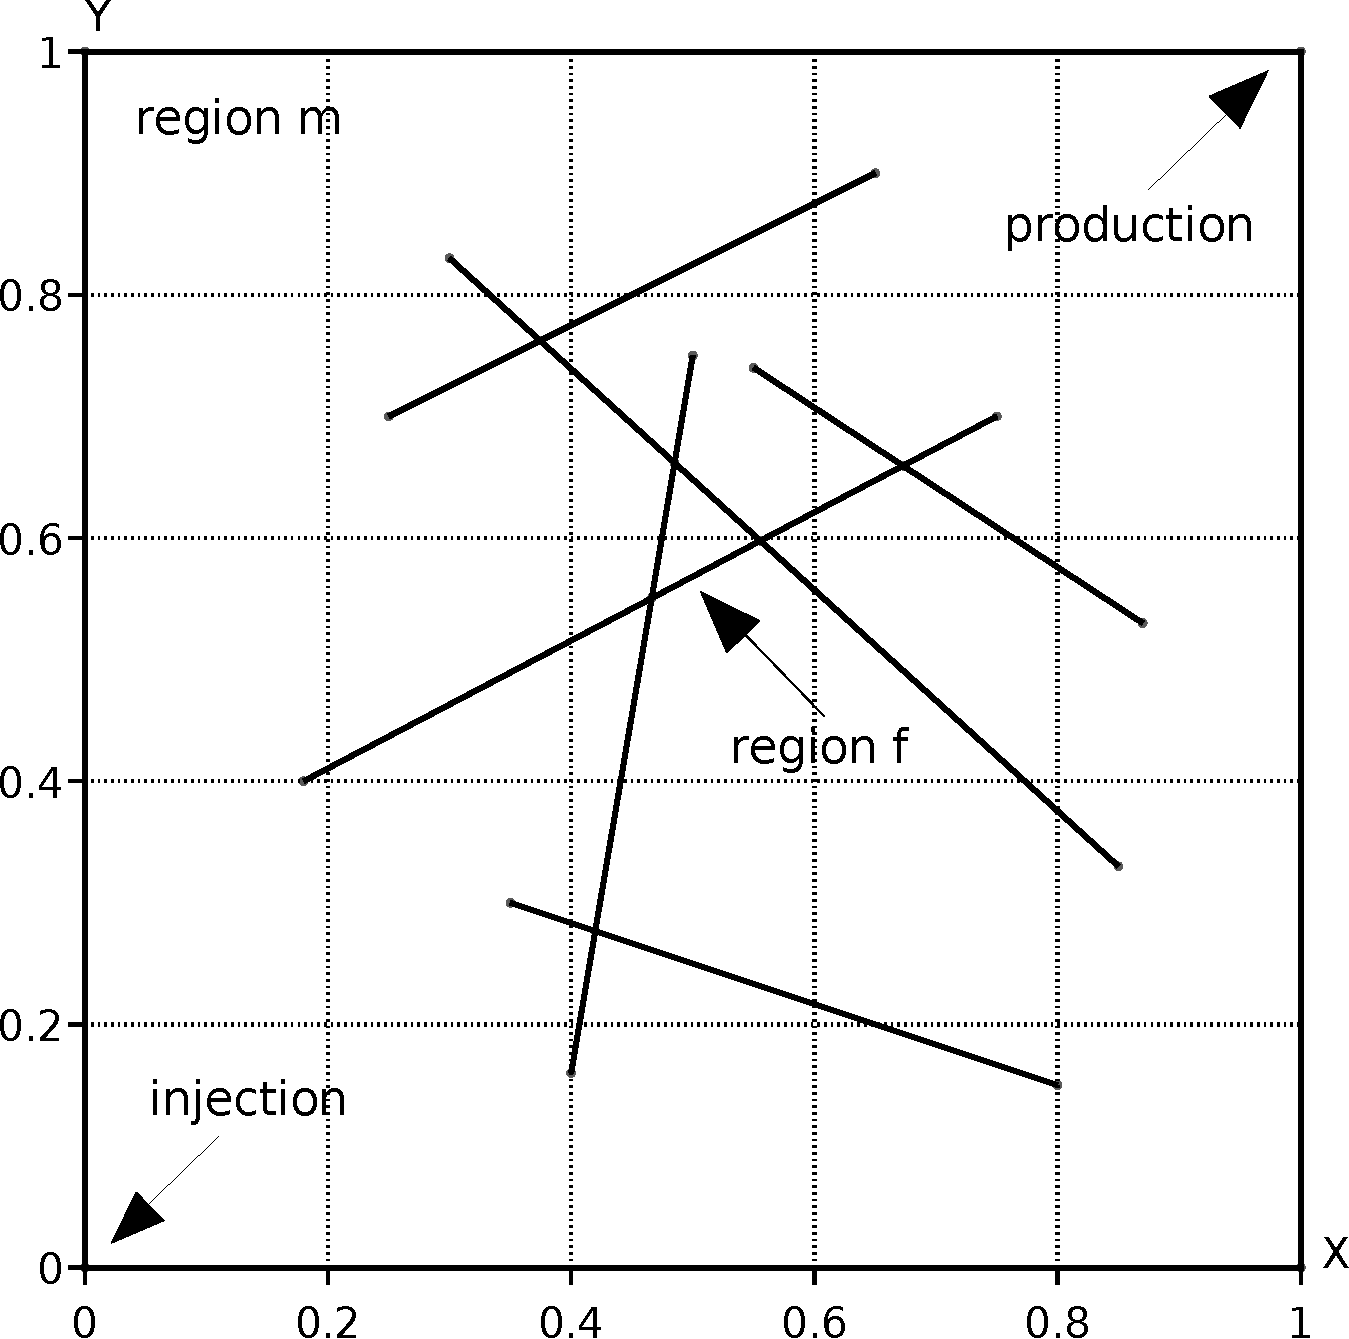
\includegraphics[width=.9\linewidth,center]{verif/firooz-geom.pdf} 
\caption{هندسه مسئله}
\label{fig:4firoozprob-geo}
\end{subfigure}
\begin{subfigure}{0.5\textwidth}
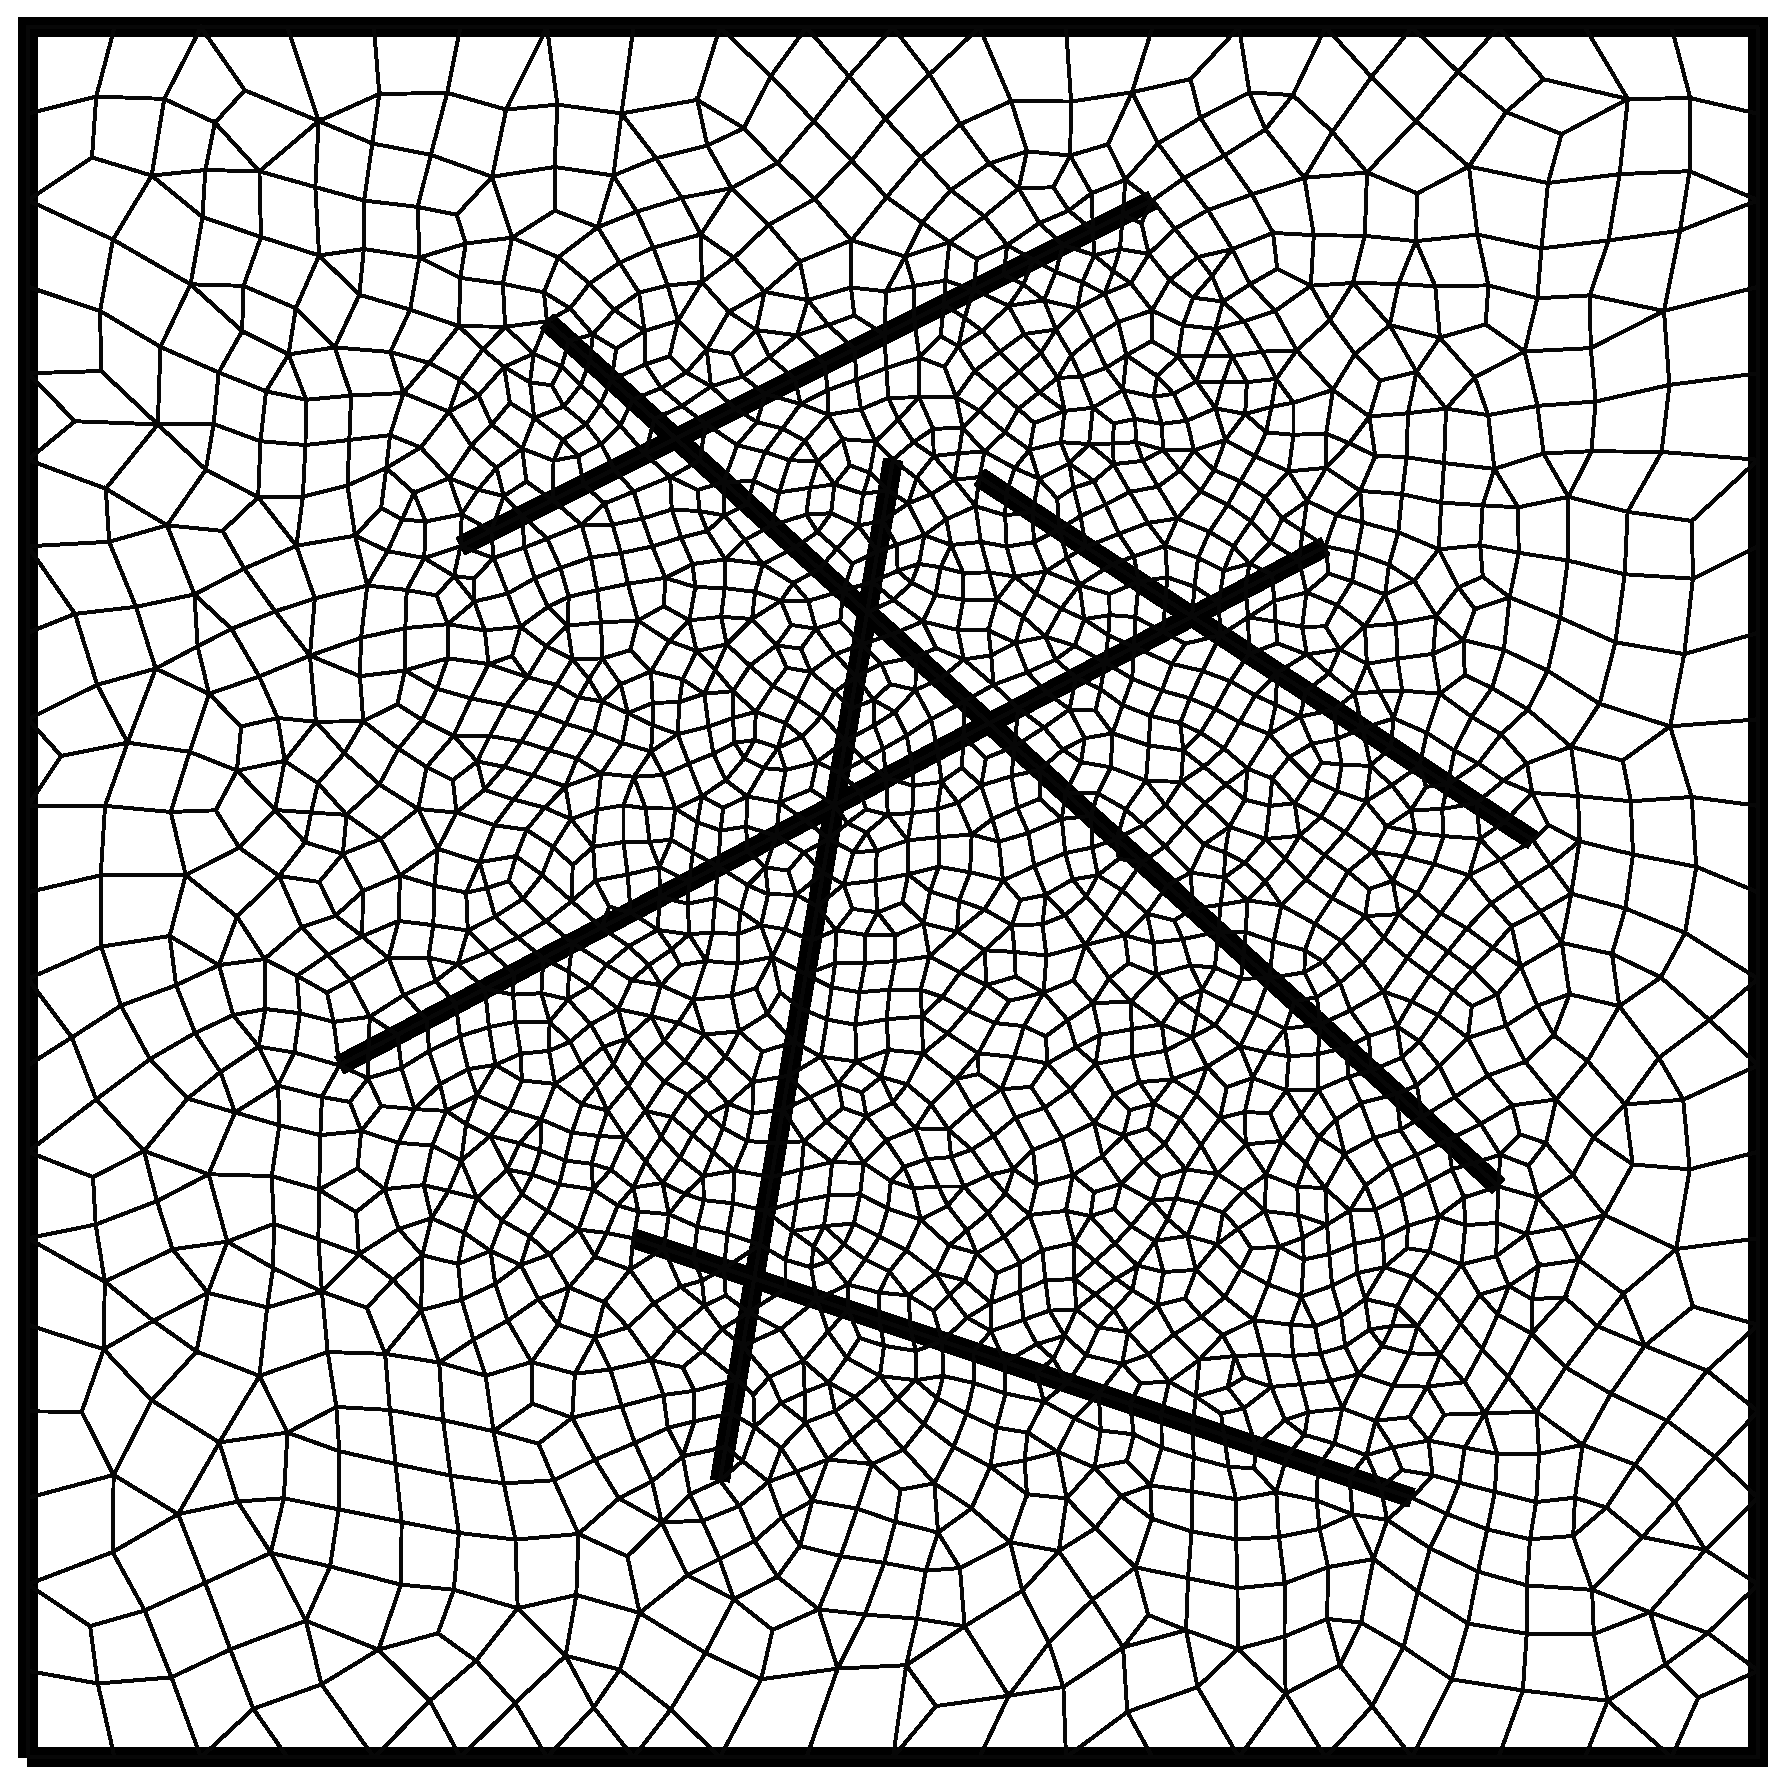
\includegraphics[width=.9\linewidth,center]{verif/firooz-mesh.eps} 
\caption{مش محاسباتی استفاده شده برای حل مسئله}
\label{fig:4firoozprob-mesh}
\end{subfigure}
\caption[هندسه و مش مسئله سوم]{هندسه و مش مسئله سوم. در این مسئله ۶ ترک در محیطی به ابعاد $1\times 1$ قرار دارند.}
\label{fig:4firoozprob} \vspace{1cm}
%-------------------figure for curves----------------------------------------------------------%------------------------------------------------------------------------------------------------x
\begin{subfigure}{0.5\textwidth}
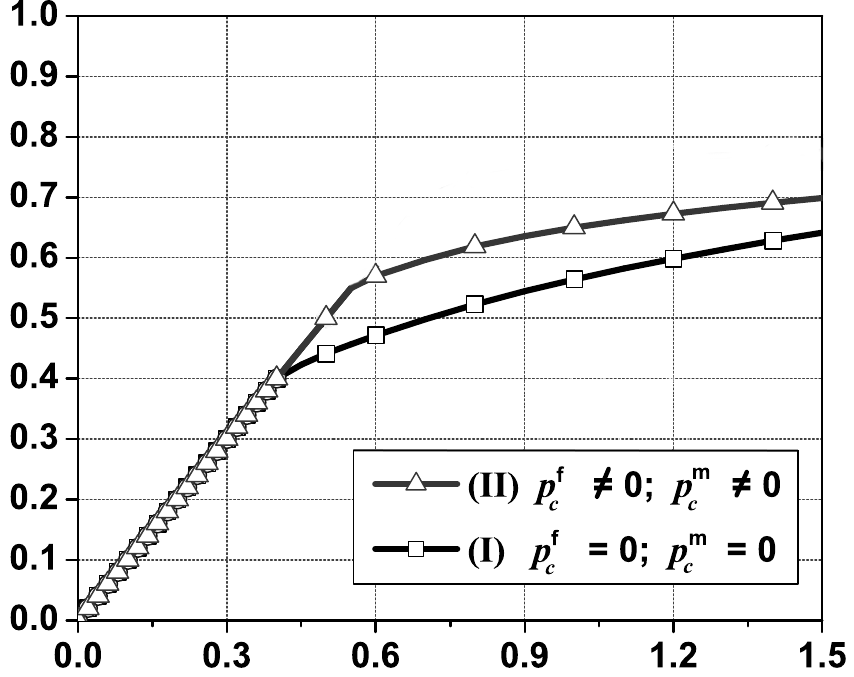
\includegraphics[width=.9\linewidth,center]{verif/firooz-curve.png} 
\caption{پاسخ مرجع \cite{hoteitf}}
\label{fig:4firoozcurve-him}
\end{subfigure}
\begin{subfigure}{0.5\textwidth}
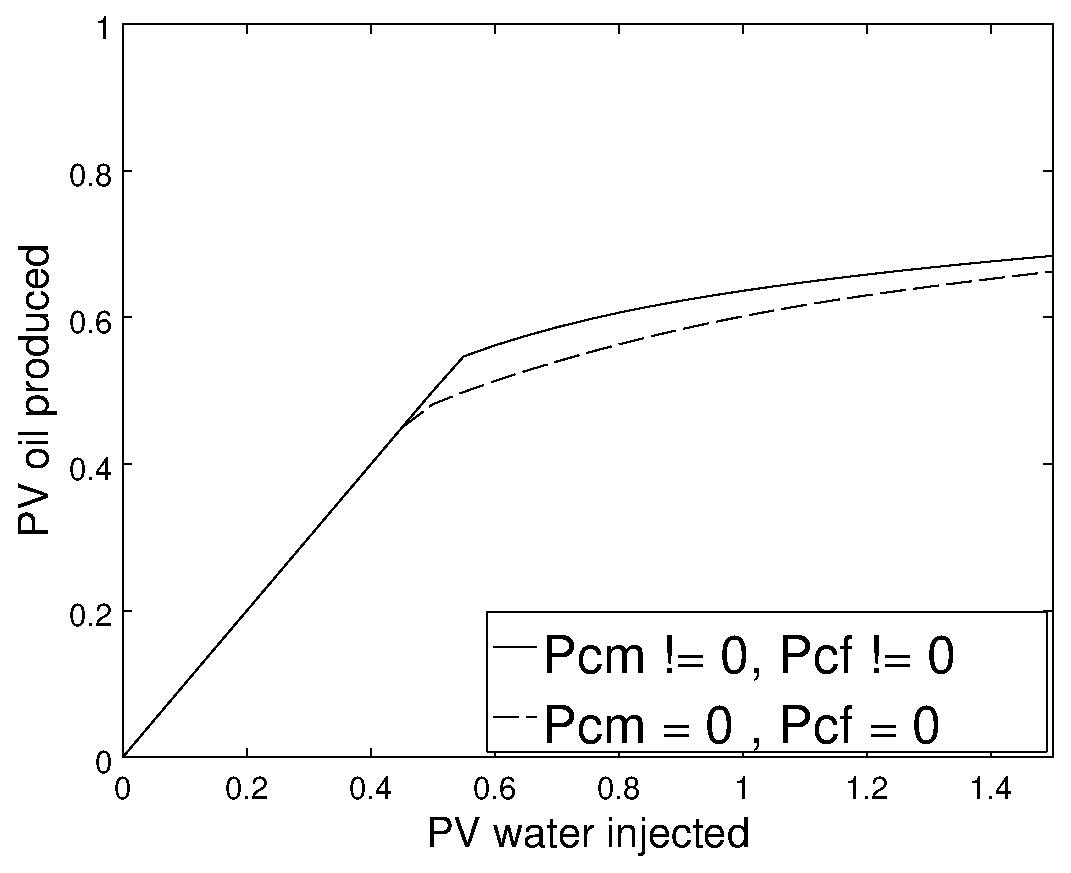
\includegraphics[width=.9\linewidth,center]{verif/firooz-me-curve.eps} 
\caption{پاسخ محاسبه شده توسط روش این پروژه}
\label{fig:4firoozcurve-me}
\end{subfigure}
\caption[منحنی آب تزریقی، نفت برداشتی برای مسئله سوم]{منحنی آب تزریقی، نفت برداشتی برای مسئله سوم. واحد تزریق و برداشت حجم بدون بعد ناحیه متخلخل است.}
\label{fig:4firoozcurve}
\end{figure}

%-------------------figure for results----------------------------------------------------------%------------------------------------------------------------------------------------------------x

\begin{figure}
\begin{subfigure}{0.5\textwidth} %%%% 25pv no cappil
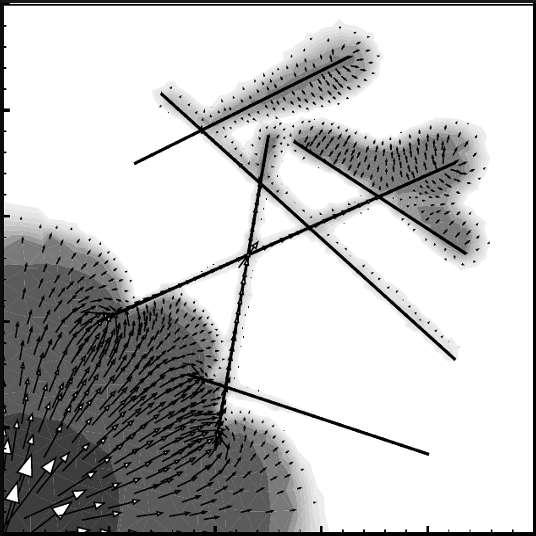
\includegraphics[width=.65\linewidth,center]{verif/firooz-25n.jpg} 
\end{subfigure}
\begin{subfigure}{0.5\textwidth} %    
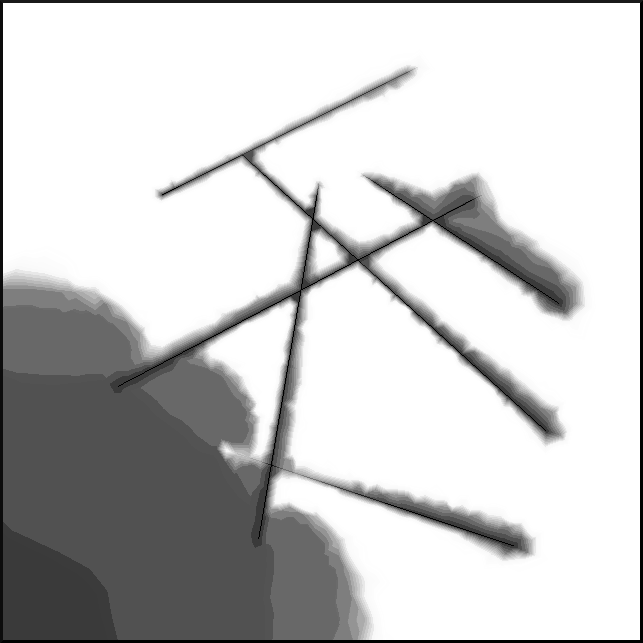
\includegraphics[width=.65\linewidth,center]{verif/firooz-me-25n.png}
\end{subfigure}
\begin{subfigure}{0.5\textwidth} %%%% 50pv no cappil
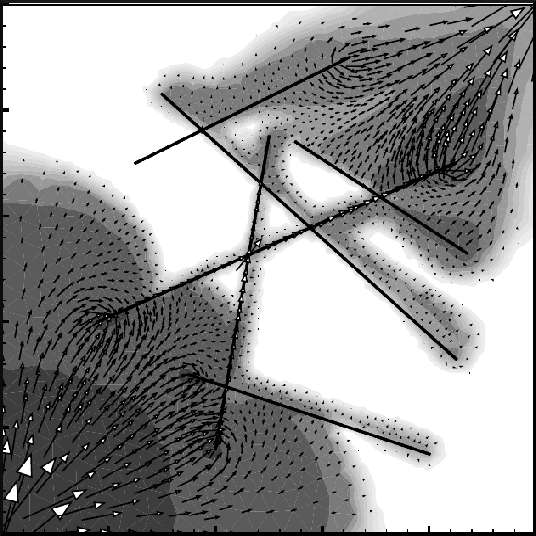
\includegraphics[width=.65\linewidth,center]{verif/firooz-50n.jpg} 
\end{subfigure}
\begin{subfigure}{0.5\textwidth} %
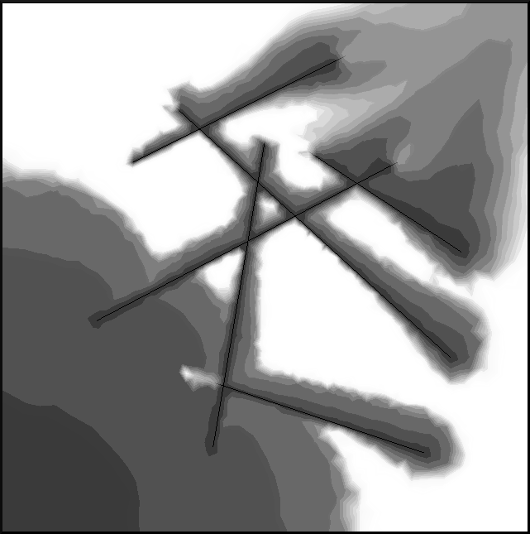
\includegraphics[width=.65\linewidth,center]{verif/firooz-me-50n.png} 
\end{subfigure}
\begin{subfigure}{0.5\textwidth} %%%% 25pv cappil
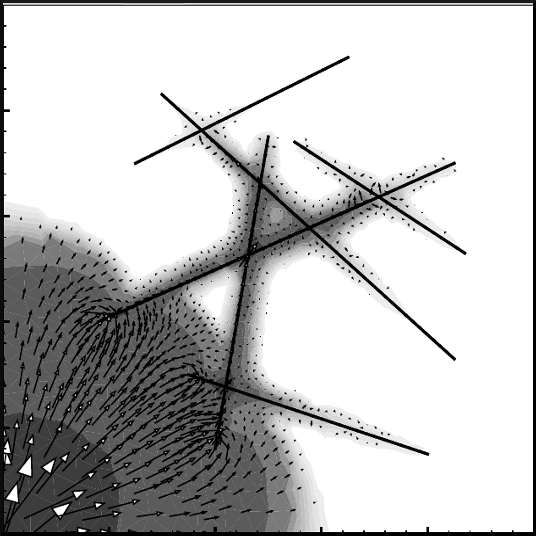
\includegraphics[width=.65\linewidth,center]{verif/firooz-25c.jpg} 
\end{subfigure}
\begin{subfigure}{0.5\textwidth} %
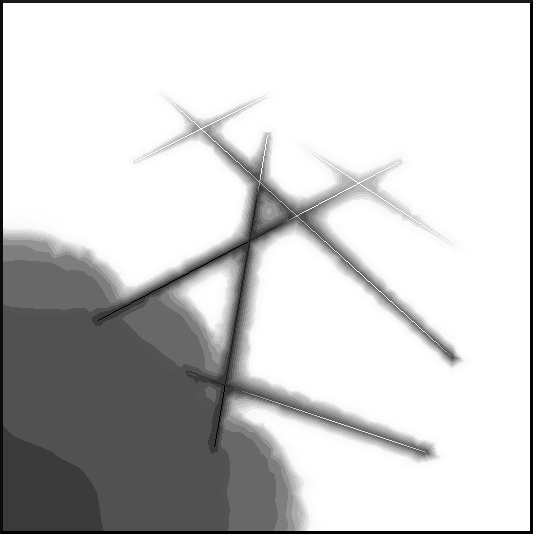
\includegraphics[width=.65\linewidth,center]{verif/firooz-me-25c.png} 
\end{subfigure}
\begin{subfigure}{0.5\textwidth} %%%% 50pv cappil
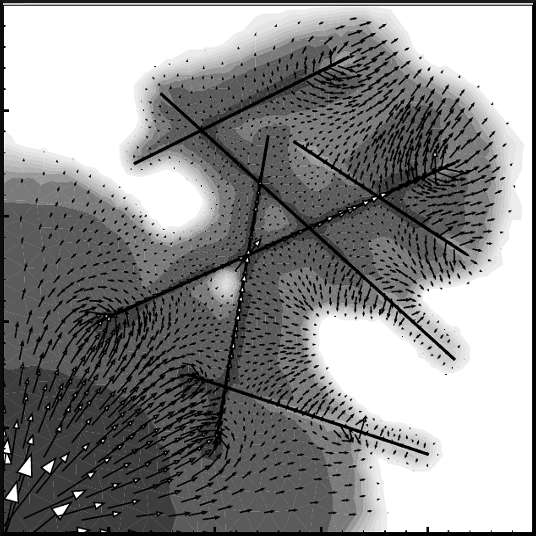
\includegraphics[width=.65\linewidth,center]{verif/firooz-50c.jpg} 
\end{subfigure}
\begin{subfigure}{0.5\textwidth} %
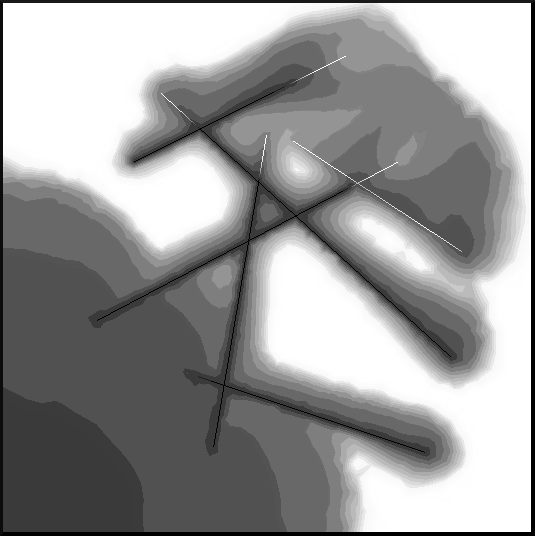
\includegraphics[width=.65\linewidth,center]{verif/firooz-me-50c.png}
\end{subfigure}
\begin{subfigure}{0.5\textwidth} %%%% bar
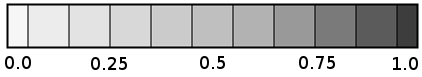
\includegraphics[width=.8\linewidth,center]{verif/firooz-bar.png} 
\caption{پاسخ مرجع \cite{hoteitf}}
\label{fig:4firoozres-him}
\end{subfigure}
\begin{subfigure}{0.5\textwidth} %

\includegraphics[width=.8\linewidth,center]{verif/firooz-me-bar.png}
\caption{پاسخ محاسبه شده توسط روش این پروژه}
\label{fig:4firoozres-me}
\end{subfigure}
\caption[پروفیل اشباع آب در حالات مختلف برای مسئله سوم]{پروفیل اشباع آب در حالات مختلف برای مسئله سوم. اشکال از بالا به پایین تزریق $25 PV$ بدون فشار مویینگی، تزریق $50 PV$ بدون فشار مویینگی، تزریق $25 PV$ با فشار مویینگی و تزریق $50 PV$ با فشار مویینگی را نمایش می‌دهند. }
\label{fig:4firoozres}
\end{figure}

%----------------------------------------------------------------------------------------ی
%----------------------------------------------------------------------------------------ی
%                                      قسمت چهارم: نتیجه‌گیری
%----------------------------------------------------------------------------------------ی
%----------------------------------------------------------------------------------------ی
\section{جمع‌بندی}
در این قسمت سه مثال عددی از مراجع \cite{vandujanal,vandujthes,basthabil,bastn,karimi1,hoteitf} حل نمودیم تا صحت کد محاسباتی نوشته شده در این پروژه را بررسی کنیم. در مسئله اوّل توانایی کد در مدل کردن ناهمگنی فشار مویینگی با شبیه‌سازی نفوذ آب از یک ناحیه با فشار مویینگی کم به ناحیه دیگر با فشار مویینگی بالا بررسی شد. در مسئله دوّم مدل‌کردن جاذبه و ناهمگنی فشار مویینگی با شبیه‌سازی نفوذ سیال \text‌لاتین{DNAPL} در یک ناحیه پر از آب بررسی شد. در مسئله سوم توانایی کد در مدل‌کردن ترک‌ها با شبیه‌سازی تزریق و برداشت آب به یک مخزن ترک‌دار بررسی شد. در تمامی مسائل نتایج به دست‌آمده از کد محاسباتی تطابق خوبی با پاسخ‌های آورده شده از مراجع داشتند. این نشان می‌دهند که کد محاسباتی به درستی پیاده‌سازی شده‌است.

